\section{$p$-adaptivity}
\label{sec:p-adaptivity}
In the process of FEM, or DGFEM usage, the domain $\Omega$ is 
first approximated by a suitable (often polygonal) domain $\Omega_h$. This is one of the so-called
{\em variational crimes} -- departures from the ``mathematically clean'' 
variational framework -- since $\Omega_h \not \subset \Omega$ and the solution 
or other functions from the weak formulation are not defined
where they are to be approximated or evaluated. In practice these crimes are often
hard to avoid. In this work, the domain $\Omega$, and its approximation used in computations $\Omega_h$ will be both denoted $\Omega$.

\subsection{Higher-order finite element space}

Let the domain $\Omega$ be covered with a mesh $\Tau_{h} = 
\{ K_1,$ $K_2, \dots, K_M \}$ where the elements $K_m$ carry arbitrary
polynomial degrees $1 \leq p_m$, $m = 1, 2, \dots, M$. The broken Sobolev space 
$H^1\lo\Omega,\mc{T}_h\ro$ is now approximated by a space of picewise-polynomial functions
\bd
  V_{h} = \{ v \in L^2(\Omega); \ v|_{K_m} \in P^{p_m}(K_m)\ \mbox{for all}\ 1 \leq m \leq M \}
\ed
where $P^{p}$ is defined as
\bd
P^{p} = \mbox{span}\{\sum_{0\leq i, j \leq p}\alpha_i\ x_1^i\ x_2^i,\ \ \alpha_i\in\mathbb{R} \}\
\ed
in case of triangles and
\bd
P^{p} = \mbox{span}\{\sum_{\substack{0\leq i, j \leq p \\i+j\leq p}}\alpha_i\ x_1^i\ x_2^i,\ \ \alpha_i\in\mathbb{R} \}\
\ed
in case of quadrilaterals.

\paragraph{}
In discontinuous Galerkin method, there is no difference between basis functions that logically belong to vertices, edges, or volumes. They are all treated as basis functions that belong to a vertex volume. Also the name (vertex-, edge- basis functions) is dropped and only the generic term \emph{basis functions} is used. The next section shows one possible way of constructing basis functions for the discontinuous Galerkin method.

\subsection{Hierarchic shape functions}
\label{sec:hierarchic}

Hierarchic shape functions are constructed in such a way that the basis
${\cal B}^{p+1}$ of the polynomial space $P^{p+1}(K)$ is obtained from
the basis ${\cal B}^p$ of the polynomial space $P^p(K)$ by adding new
shape functions only. This is essential for $p$- and $hp$-adaptive finite 
element codes since one does not have to change the shape functions
completely when increasing the degree of polynomial approximation. 
In this section we will describe the popular \emph{Lagrange-based}
hierarchic shape functions.

\begin{definition}[Legendre polynomials]
We define the \emph{Legendre polynomials} of degree $k$ as
\bd
{\rm L}_k(x) = \frac{1}{2^kk!}\frac{{\rm d}^k}{{\rm d}x^k}(x^2-1)^k, \ \ \ k = 0,1,2,\dots
\ed
\end{definition}

The set of Legendre polynomials forms an orthonormal basis of the space $L^2(-1,1)$.

\paragraph{Quadrilaterals}
On quadrilaterals, the set of shape functions is the product of Legendre polynomials. Displayed are basis functions up to the degree 3.
\begin{figure}[H]
\begin{center}
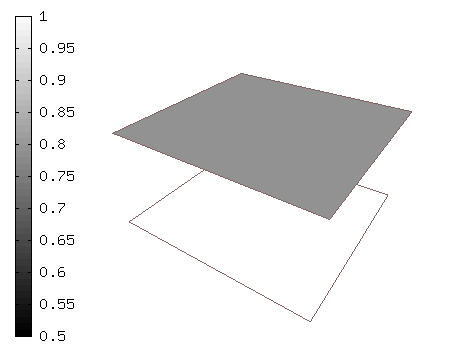
\includegraphics[width=4.4cm]{minor_examples/BasisFunctions001}
\\
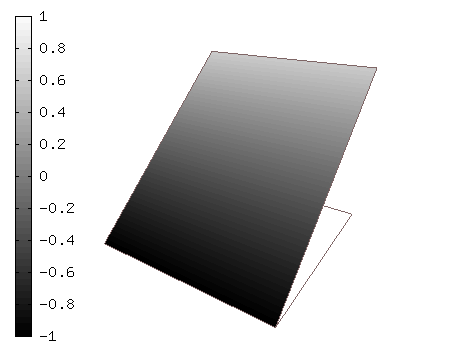
\includegraphics[width=4.4cm]{minor_examples/BasisFunctions002}
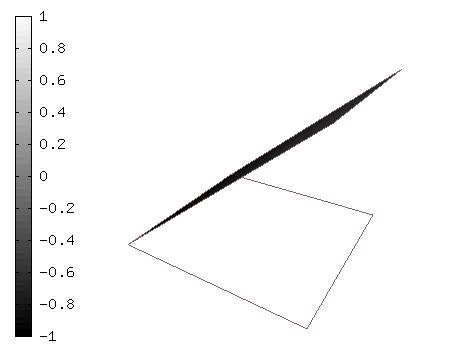
\includegraphics[width=4.4cm]{minor_examples/BasisFunctions005}
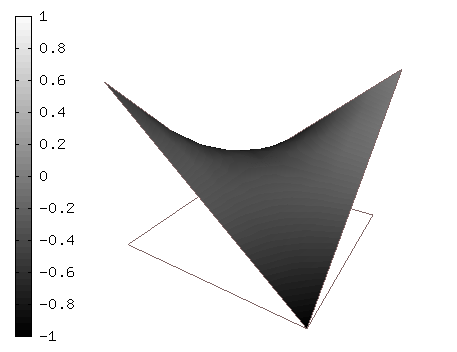
\includegraphics[width=4.4cm]{minor_examples/BasisFunctions006}
\end{center}
\caption{Shape functions - degree 0 top, degree 1 bottom}
\vspace{-7mm}
\label{bubbleshape1q}
\end{figure}

\begin{figure}[H]
\begin{center}
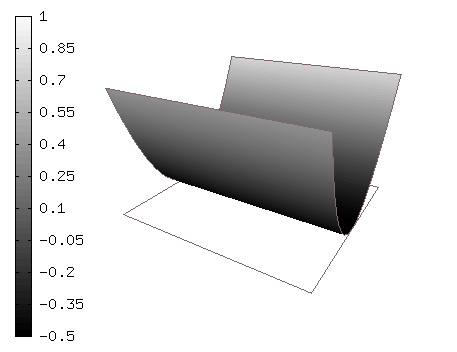
\includegraphics[width=4.4cm]{minor_examples/BasisFunctions003}
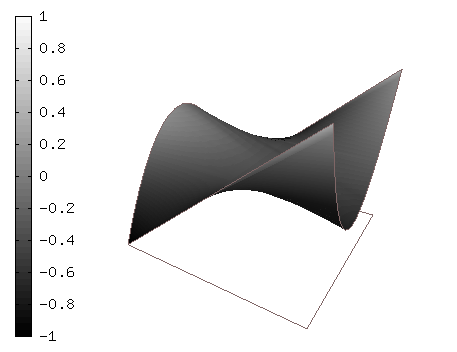
\includegraphics[width=4.4cm]{minor_examples/BasisFunctions007}
\\
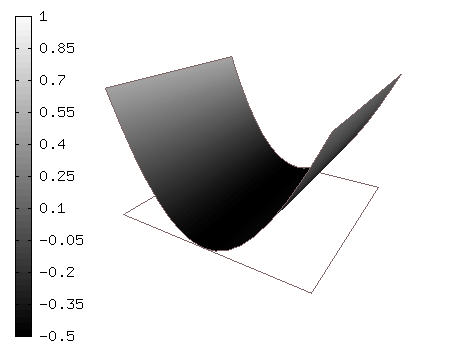
\includegraphics[width=4.4cm]{minor_examples/BasisFunctions009}
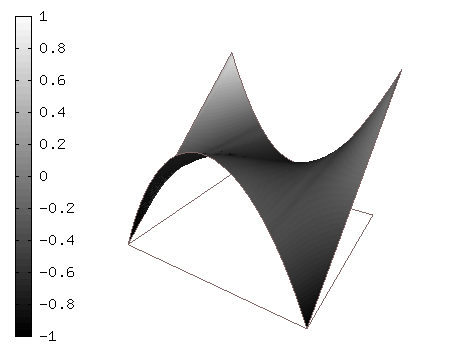
\includegraphics[width=4.4cm]{minor_examples/BasisFunctions010}
\end{center}
\caption{Shape functions - degree 2}
\vspace{-7mm}
\label{bubbleshape2q}
\end{figure}

\begin{figure}[H]
\begin{center}
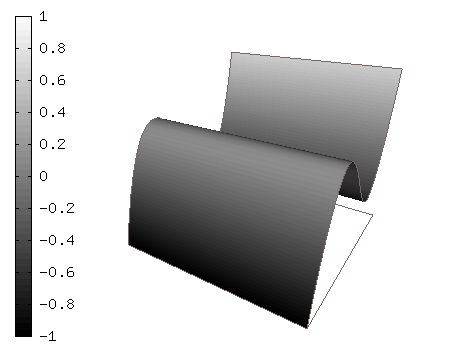
\includegraphics[width=4.4cm]{minor_examples/BasisFunctions004}
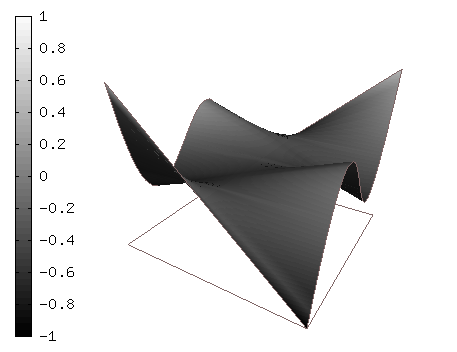
\includegraphics[width=4.4cm]{minor_examples/BasisFunctions008}
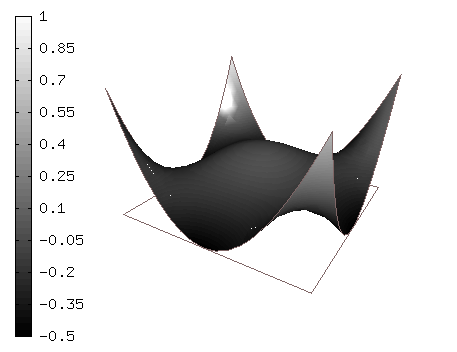
\includegraphics[width=4.4cm]{minor_examples/BasisFunctions011}
\\
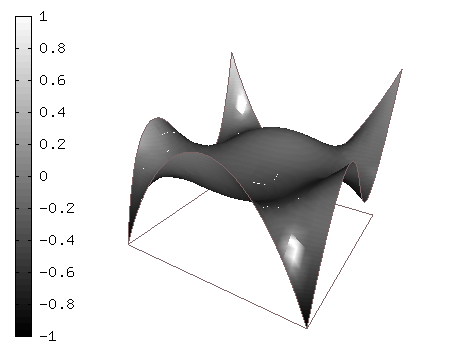
\includegraphics[width=4.4cm]{minor_examples/BasisFunctions012}
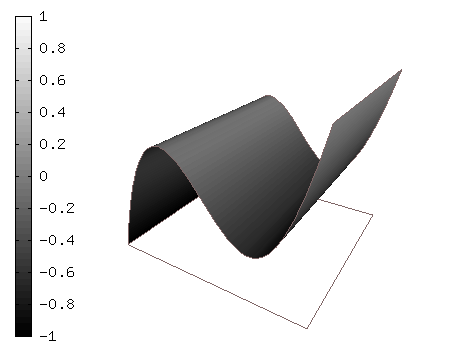
\includegraphics[width=4.4cm]{minor_examples/BasisFunctions013}
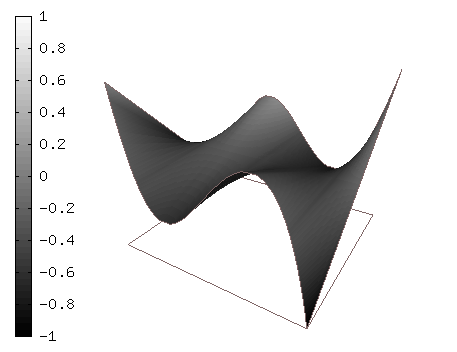
\includegraphics[width=4.4cm]{minor_examples/BasisFunctions014}
\\
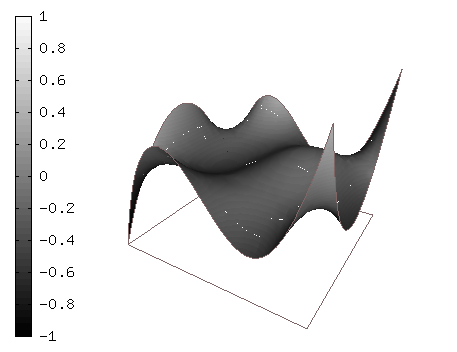
\includegraphics[width=4.4cm]{minor_examples/BasisFunctions015}
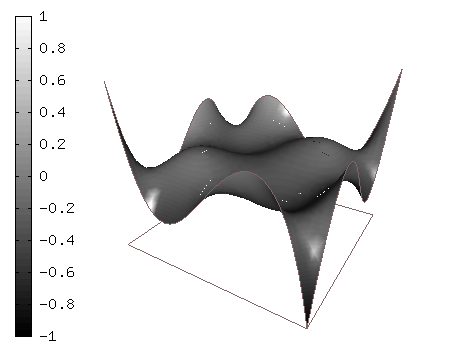
\includegraphics[width=4.4cm]{minor_examples/BasisFunctions016}
\end{center}
\caption{Shape functions - degree 3}
\vspace{-7mm}
\label{bubbleshape3q}
\end{figure}

\paragraph{Triangles}
Situation on triangles is a bit more complicated. Since the number of basis functions spanning the space of polynomials of certain degree is not the same as on quadrilaterals, the set of shape functions can not be the product of Legendre polynomials. In the construction of the set, the following definition will be used.
\begin{definition}[Affine coordinates]
\emph{Barycentric coordinates} on the triangular reference domain $\hat{K}$ (Figure \ref{refdomain})
are defined as
\bd
  \lambda_1(\xi_1,\xi_2)=\frac{\xi_2+1}{2},\ 
  \lambda_2(\xi_1,\xi_2)=-\frac{\xi_1+\xi_2}{2},\ 
  \lambda_3(\xi_1,\xi_2)=\frac{\xi_1+1}{2}
\ed
\end{definition}
Now the basis functions are defined in the following way:
\be
L_{ij}^{tri} = {\rm L}_i(\lambda_3(x,y) - \lambda_2(x,y)) \cdot {\rm L}_j(\lambda_2(x,y) - \lambda_1(x,y)),
\ee
the resulting set is then $L^{tri}_p = \left\{L_{ij}^{tri},\ i,j = 0, ..., p\right\}$, where $p$ represents the highest polynomial degree we use for approximation.
Figures of the set for $p = 3$ follows.
\begin{figure}[H]
\begin{center}
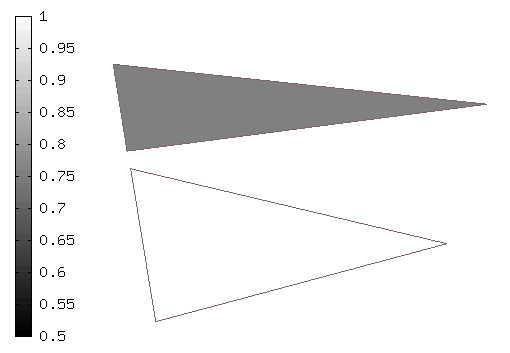
\includegraphics[width=4.4cm]{minor_examples/BasisFunctions017}
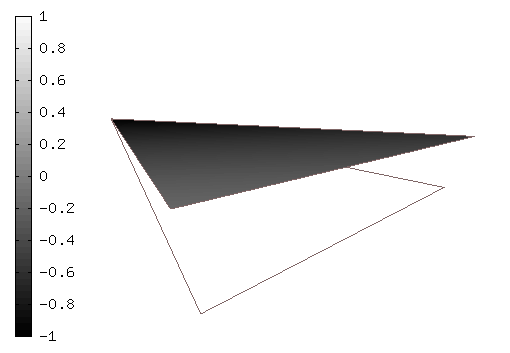
\includegraphics[width=4.4cm]{minor_examples/BasisFunctions018}
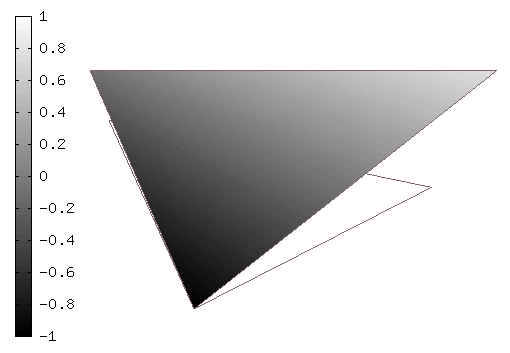
\includegraphics[width=4.4cm]{minor_examples/BasisFunctions019}
\end{center}
\caption{Shape functions - degree 0 on the left, degree 1 rest}
\vspace{-7mm}
\label{bubbleshape1t}
\end{figure}

\begin{figure}[H]
\begin{center}
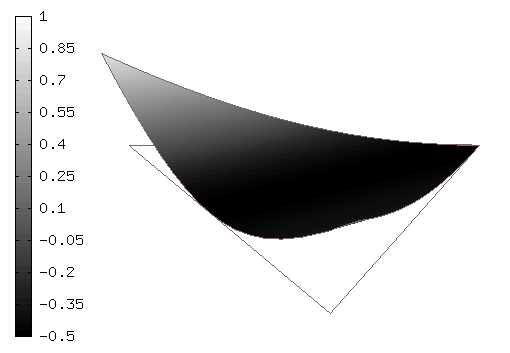
\includegraphics[width=4.4cm]{minor_examples/BasisFunctions020}
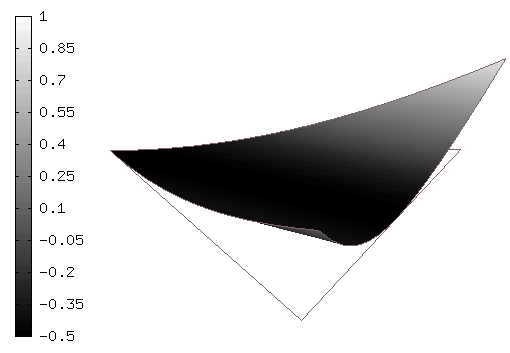
\includegraphics[width=4.4cm]{minor_examples/BasisFunctions021}
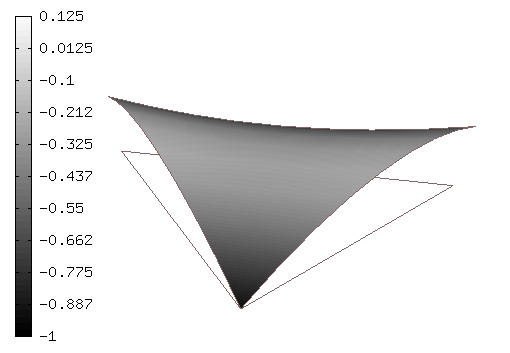
\includegraphics[width=4.4cm]{minor_examples/BasisFunctions024}
\end{center}
\caption{Shape functions - degree 2}
\vspace{-7mm}
\label{bubbleshape2t}
\end{figure}

\begin{figure}[H]
\begin{center}
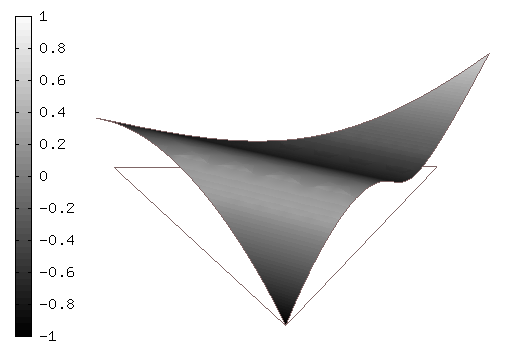
\includegraphics[width=4.4cm]{minor_examples/BasisFunctions023}
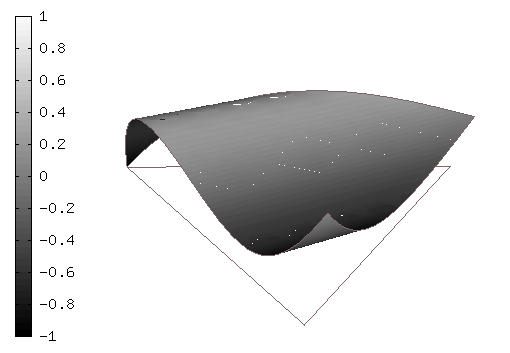
\includegraphics[width=4.4cm]{minor_examples/BasisFunctions022}
\\
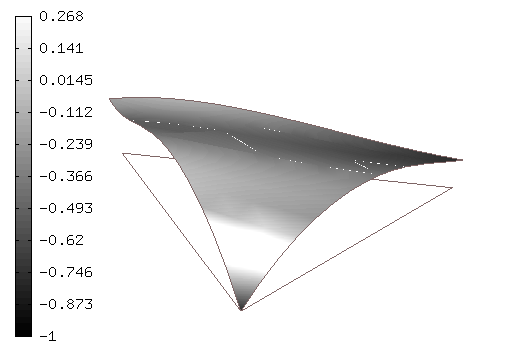
\includegraphics[width=4.4cm]{minor_examples/BasisFunctions025}
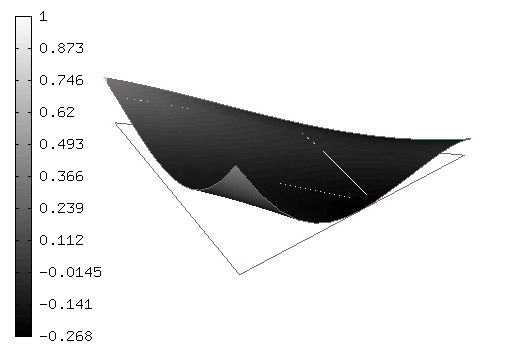
\includegraphics[width=4.4cm]{minor_examples/BasisFunctions026}
\end{center}
\caption{Shape functions - degree 3}
\vspace{-7mm}
\label{bubbleshape3t}
\end{figure}

\paragraph{}
\begin{proposition}
The shape functions described above, both on quadrilaterals, and on triangles constitute
a hierarchic basis of the space $P^{p_m}(\hat{K})$
\end{proposition}
\begin{proof}
The complete proof can be found in \cite{solin1}. Briefly, the following 
must be verified:
\vspace{-2ex}
\begin{enumerate}
\parskip=0pt %\itemsep=0pt
\item Are all the shape functions linearly independent?
\item Do they all belong to the space $P^{p_m}(\hat{K})$?
\item Matches their number the dimension of the space $P^{p_m}(\hat{K})$?
\end{enumerate}
\end{proof}

\subsection{Higher-order numerical quadrature}
\label{sec:numquad}

Most commonly, the integrals in (\ref{stiffmat}), (\ref{rhs}) are evaluated
numerically by the \emph{Gaussian quadrature}. The $k$-point Gaussian quadrature
rule on the domain $\hat{K}$ has the form
\be \label{gaussrule}
  \int_{\hat{K}} g(\xi) \mbox{d}\xi \approx \sum_{i=1}^k w_{k,i} g(\xi_{k,i})
\ee
where $g$ is a bounded continuous function, $\xi_{k,i} \in \hat{K}, i = 1,2,\dots,k$ are
the integration points and $w_{k,i} \in \mathbb{R}$ are the integration weights.
The sum of the integration weights must be equal to the area of $\hat{K}$, so that
the rule (\ref{gaussrule}) is exact for constants. If the points and weights are
chosen carefully, the formula (\ref{gaussrule}) can be exact for polynomials
up to a certain degree $q > 0$.

In 1D the integration points are roots of the Legendre polynomials. Also in 2D
it is quite easy to find the integration points and weights for low-degree polynomials
ocurring in traditional linear FEM. For higher-degree polynomials, however, the
task of finding optimal Gaussian quadrature rules presents a complex non-linear
optimization problem with many open questions left. Optimal integration points
and weights are known on $\hat{K}$ for polynomials up to degree 10. Suboptimal (with
more points than necessary) rules have been found for polynomials up to degree 20.
Complete integration tables along with more information on this subject 
can be found in \cite{solin1}.
